\documentclass{article}
\linespread{1.3}
\usepackage[margin=50pt]{geometry}
\usepackage{amsmath, amsthm, amssymb, amsthm, tikz, fancyhdr, graphicx}
\pagestyle{fancy}
\renewcommand{\headrulewidth}{0pt}
\newcommand{\changefont}{\fontsize{15}{15}\selectfont}

\fancypagestyle{firstpageheader}
{
  \fancyhead[R]{\changefont Michael Huang \\ CFRM 420 \\ Homework 7}
}

\begin{document}

\thispagestyle{firstpageheader}

\section*{1.}
{\Large 

\subsection*{(a)}

We implement this in R. The t-test assumes that the sample comes from a student's t-distribution, which also assumes that the variance is unknown.
% but that the monthly log returns are not normal. 
% what does this mean?
\\
We get the following results: \\ 
t-statistic: 2.9423 \\
p-value: 0.006696 \\ \\
Since our p-value of $0.006696 < 0.05$, we end up rejecting the null hypothesis that $\mu_1 = \mu_2$ at a 5\% significance level; i.e. the difference in the means of the two series is statistically significant, in fact, $\mu_1$ is statistically significantly greater than $\mu_2$.

\subsection*{(b)}

We implement this in R, and get the following results: \\ 
t-statistic = -2.1296 \\
p-value = 0.05662 \\ \\ 
Since our p-value of $0.05662 > 0.05$, we end up failing to reject the null hypothesis that $\mu_2 = 0.16$ at a 5\% significance level; i.e. the difference between $\mu_2$ and $0.16$ is not statistically significant.
\newpage

}

\section*{2.}
{\Large 
\subsection*{(a)}

\begin{itemize}
  \item Let $T = |S|$ and $t = |s|$. Under the null hypothesis, let the distribution of $T$ have cdf $F_T$, then $P = 1 - F_T(T).$
\end{itemize}
We define the variables in accordance with the given setup. Logically, with a two-sided test, with the cdf of $T$, the function is symmetric as defined.

% we have $P$ as $\mathbb{P}(S > s)$ or $\mathbb{P}(S < s)$, which logically equates to the probability that the test value does not lie within the range, which is simply just the probability not covered by the cdf, which is equivalent to $P = 1 - F_T(T).$
\begin{itemize}
  \item Then $\mathbb{P}(P \leq x) = 1 - \mathbb{P}(F_T(T) \leq 1 - x), 0 < x < 1$
\end{itemize}
% In the same way, taking the probability that the $P$ is contained within the range of some probability $x$ is going to be $1 - F_T(T)$, which in this case will be the probability that the cdf is not contained within the cdf of $x$. 
We can compute this by definition of the cdf: \\
$\mathbb{P}(P \leq x) = \mathbb{P}(1-F_T(T) \leq x)$ \\
$= \mathbb{P}(F_T(T) \geq 1-x)$ \\
$= 1 - \mathbb{P}(F_T(T) \leq 1-x)$ as we aimed to find. We also know the range of $x$ is 0 to 1 since the cdf goes from from 0 to 1.
\begin{itemize}
  \item This implies $\mathbb{P}(P \leq x) = 1 - F_T(F_T^{-1}(1-x)),$ where $F_T^{-1}$ is the inverse function of $F_T$ or the quantile function of $T$. 
\end{itemize}
In the same way as before, we can calculate this using the definition of the cdf: \\
$\mathbb{P}(F_T(T) \leq 1 - x) = F_T(F_T(T) \leq 1-x)$ \\
We can then reconstruct the cdf using the definition of the quantile function as the inverse of the cdf: \\
$F_T(T) \leq 1 - x = F_T^{-1}(1-x)$ \\
which then allows us to substitute and find that \\
$\mathbb{P}(F_T(T) \leq 1 - x) = F_T(F_T^{-1}(1-x))$

% We take the cdf of the inverse, which gives us the quantile function of the normal.
\begin{itemize}
  \item Therefore, the $p-$value has distribution $P \sim$ Uniform(0,1).
\end{itemize}
Simplifying from the above equation simply gives us that $\mathbb{P}(P \leq x) = 1 - 1 - x = x$ as the representation of the distribution, and as we know $x$ is in the range 0 to 1, we can say that $P$ simply is $x$ in this range, or the uniform distribution in this range $\text{Uniform}(0,1)$.

\subsection*{(b)}

We implement this test in R and verify that this indeed does follow the normal distribution: 
\begin{figure}[h!]
  \centering
  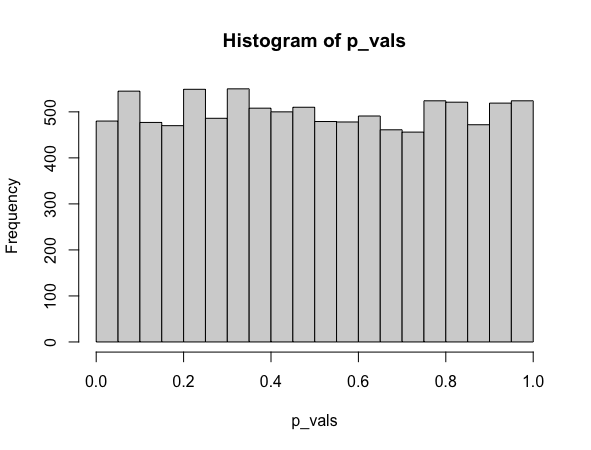
\includegraphics[width=325pt]{hw7_2b.png}
\end{figure}

\subsection*{(c)}

We implement this in R. We see that the distribution is heavily skewed right, with more values to the left side.
\begin{figure}[h!]
  \centering
  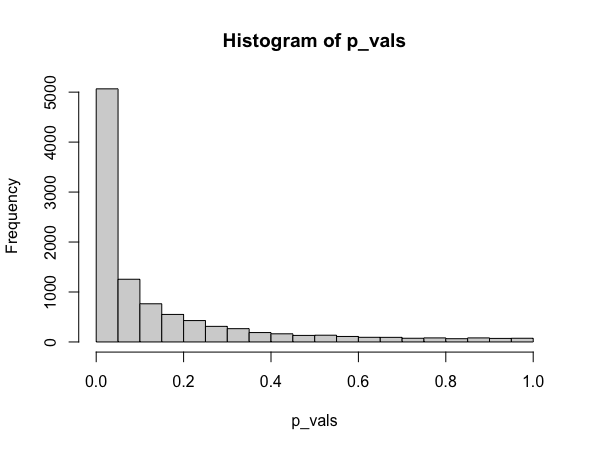
\includegraphics[width=325pt]{hw7_2c.png}
\end{figure}

\subsection*{(d)}

We implement this in R. We see that the distribution is still skewed right, with more values to the left side, but not a severely as before.
\begin{figure}[h!]
  \centering
  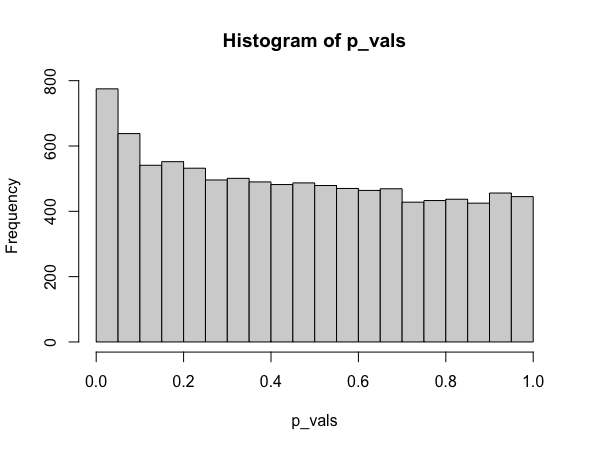
\includegraphics[width=305pt]{hw7_2d.png}
\end{figure}

\subsection*{(e)}

We implement this in R. We see that the distribution is skewed right, with more values to the left side, to a less extreme than in part (c), but still more of an apparent trend than in part (d).
\begin{figure}[h!]
  \centering
  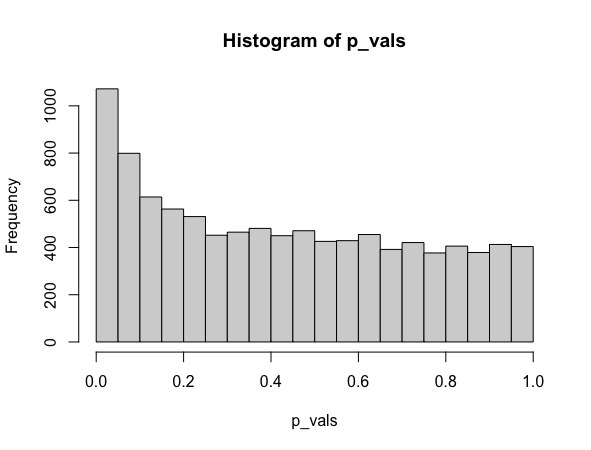
\includegraphics[width=305pt]{hw7_2e.png}
\end{figure}

\subsection*{(f)}

We implement this in R. We see that the distribution is relatively uniform, like in part (b), which is interesting for actual market data.
\begin{figure}[h!]
  \centering
  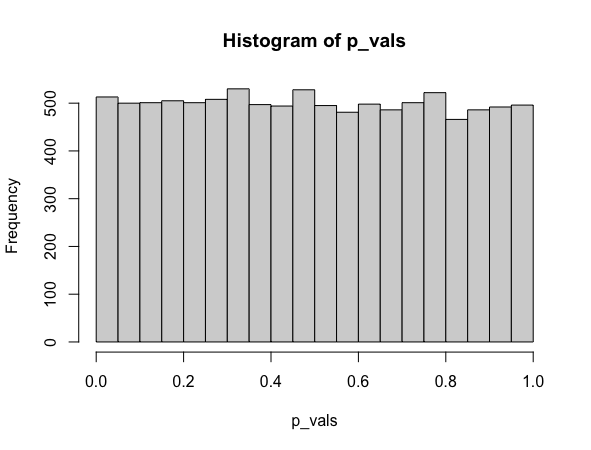
\includegraphics[width=315pt]{hw7_2f.png}
\end{figure}

\subsection*{(g)}

We implement this in R. We see that the distribution is starting to skew right and get more p-values on the left-hand side, as in part (e).
\begin{figure}[h!]
  \centering
  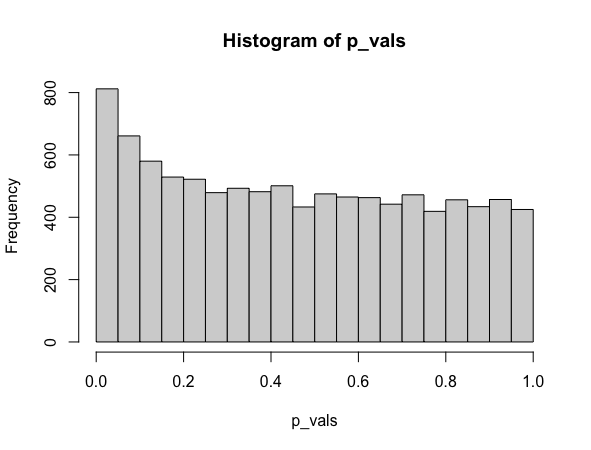
\includegraphics[width=315pt]{hw7_2g.png}
\end{figure}

}

\end{document}